\subsection{CENTRAL FUNCTIONS ON G AND FUNCTIONS ON T}

Denote by \(\mathcal{C}(\mathrm{G})\) the space of continuous complex-valued functions on G and by \(\mathcal{C}^{\infty}(\mathrm{G})\) the subspace of infinitely-differentiable functions. Then we have a sequence of inclusions

\[
\Theta (\mathrm{G}) \subset \mathscr {C} ^ {\infty} (\mathrm{G}) \subset \mathscr {C} (\mathrm{G}) \subset \mathrm{L} ^ {2} (\mathrm{G}).
\]

Denote by \(Z\Theta(G)\) , \(Z\mathcal{C}^{\infty}(G)\) , \(Z\mathcal{C}(G)\) , \(ZL^{2}(G)\) , respectively, the subspaces consisting of the central functions in these various spaces. Introduce similarly the spaces \(\Theta(T)\) , \(\mathcal{C}^{\infty}(T)\) , \(\mathcal{C}(T)\) , \(L^{2}(T)\) ; for any space E in this list, denote by \(E^{W}\) (resp. \(E^{-W}\) ) the subspace consisting of the invariant (resp. anti-invariant) elements for the operation of the Weyl group W. We have a commutative diagram

\[
\begin{array}{c c c} \mathsf {Z C} (\mathsf {G}) & \stackrel {{a _ {c}}} {{\longrightarrow}} & \mathcal {C} (\mathsf {T}) ^ {\mathsf {W}} \\ \uparrow & & \uparrow \\ \mathsf {Z C} ^ {\infty} (\mathsf {G}) & \stackrel {{a _ {\infty}}} {{\longrightarrow}} & \mathcal {C} ^ {\infty} (\mathsf {T}) ^ {\mathsf {W}} \\ \uparrow & & \uparrow \\ \mathsf {Z} \Theta (\mathsf {G}) & \stackrel {{a _ {\Theta}}} {{\longrightarrow}} & \Theta (\mathsf {T}) ^ {\mathsf {W}} \end{array}
\]

where the vertical arrows represent the canonical injections, and the maps \(a_{c}, a_{\infty}, a_{\Theta}\) are induced by the restriction map from \(\mathcal{C}(G)\) to \(\mathcal{C}(T)\) .

The maps \(a_c, a_\infty, a_\Theta\) are bijective (§2, no. 5, Cor. 1 of Prop. 5, §8, no. 3, Cor. of Prop. 5, and §7, no. 3, Cor. of Prop. 2).

Assume now that the semi-sum \(\rho\) of the positive roots belongs to X(T) and consider the map b which to every continuous function \(\varphi\) on T associates \(\varphi\cdot\mathrm{J}(\rho)\) . We have a commutative diagram

\pandocbounded{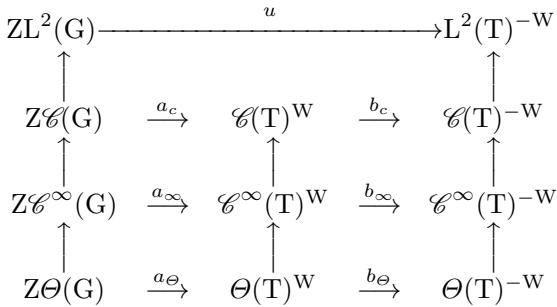
\includegraphics[keepaspectratio]{images/part003_8b0b3ceb.jpg}}

where the vertical arrows are the canonical inclusions, the maps \(b_{c}, b_{\infty}, b_{\Theta}\) are induced by b, and u extends \(b_{c} \circ a_{c}\) by continuity (§7, no. 4, Cor. 3 of Th. 2). The maps u and \(b_{\Theta}\) are bijective (loc. cit.); so is \(b_{\infty}\) (Exerc. 5); on the other hand, \(b_{c}\) is not surjective in general (Exerc. 6).

